\documentclass[a4paper,11pt]{article}
\usepackage{amsmath,amsthm,amsfonts,amssymb,amscd,amstext,vmargin,graphics,graphicx,tabularx,multicol} 
\usepackage[francais]{babel}
\usepackage[utf8]{inputenc}  
\usepackage[T1]{fontenc} 
\usepackage{pstricks-add,tikz,tkz-tab,variations}
\usepackage[autolanguage,np]{numprint} 
\usepackage{calc}
\usepackage{pifont}

\setmarginsrb{1.5cm}{0.5cm}{1cm}{0.5cm}{0cm}{0cm}{0cm}{0cm} %Gauche, haut, droite, haut
\newcounter{numexo}
\newcommand{\exo}[1]{\stepcounter{numexo}\noindent{\bf Exercice~\thenumexo} : }
\reversemarginpar

\newcommand{\bmul}[1]{\begin{multicols}{#1}}
\newcommand{\emul}{\end{multicols}}

\newcounter{enumtabi}
\newcounter{enumtaba}
\newcommand{\q}{\stepcounter{enumtabi} \theenumtabi.  }
\newcommand{\qa}{\stepcounter{enumtaba} (\alph{enumtaba}) }
\newcommand{\initq}{\setcounter{enumtabi}{0}}
\newcommand{\initqa}{\setcounter{enumtaba}{0}}

\newcommand{\be}{\begin{enumerate}}
\newcommand{\ee}{\end{enumerate}}
\newcommand{\bi}{\begin{itemize}}
\newcommand{\ei}{\end{itemize}}
\newcommand{\bp}{\begin{pspicture*}}
\newcommand{\ep}{\end{pspicture*}}
\newcommand{\bt}{\begin{tabular}}
\newcommand{\et}{\end{tabular}}
\renewcommand{\tabularxcolumn}[1]{>{\centering}m{#1}} %(colonne m{} centrée, au lieu de p par défault) 
\newcommand{\tnl}{\tabularnewline}

\newcommand{\trait}{\noindent \rule{\linewidth}{0.2mm}}
\newcommand{\hs}[1]{\hspace{#1}}
\newcommand{\vs}[1]{\vspace{#1}}

\newcommand{\N}{\mathbb{N}}
\newcommand{\Z}{\mathbb{Z}}
\newcommand{\R}{\mathbb{R}}
\newcommand{\C}{\mathbb{C}}
\newcommand{\Dcal}{\mathcal{D}}
\newcommand{\Ccal}{\mathcal{C}}
\newcommand{\mc}{\mathcal}

\newcommand{\vect}[1]{\overrightarrow{#1}}
\newcommand{\ds}{\displaystyle}
\newcommand{\eq}{\quad \Leftrightarrow \quad}
\newcommand{\vecti}{\vec{\imath}}
\newcommand{\vectj}{\vec{\jmath}}
\newcommand{\Oij}{(O;\vec{\imath}, \vec{\jmath})}
\newcommand{\OIJ}{(O;I,J)}


\newcommand{\reponse}[1][1]{%
\multido{}{#1}{\makebox[\linewidth]{\rule[0pt]{0pt}{20pt}\dotfill}
}}

\newcommand{\titre}[5] 
% #1: titre #2: haut gauche #3: bas gauche #4: haut droite #5: bas droite
{
\noindent #2 \hfill #4 \\
#3 \hfill #5

\vspace{-1.6cm}

\begin{center}\rule{6cm}{0.5mm}\end{center}
\vspace{0.2cm}
\begin{center}{\large{\textbf{#1}}}\end{center}
\begin{center}\rule{6cm}{0.5mm}\end{center}
}



\begin{document}
\pagestyle{empty}
\titre{Séance d'AP . . . : Utilisation de la calculatrice}{}{}{3ème}{}

\vspace*{0.2cm}


\setlength{\fboxrule}{2pt}
\begin{flushleft}
\framebox{\begin{minipage}{\linewidth}

\vspace*{0.2cm}

\underline{\textbf{{\large Quelques touches à connaître :}}}\\


\ding{228}

\includegraphics[scale=0.55]{moins.eps} : cette touche sert à mettre \textbf{un signe "-"} au début d'un calcul.\\


\ding{228}  
\includegraphics[scale=0.8]{sd.eps} \hspace*{0.25cm} ou \hspace*{0.25cm} 
\includegraphics[scale=0.5]{fleches.eps} : ces touches servent à passer d'une écriture décimale à une fraction irréductible.\\



\ding{228}  
\includegraphics[scale=0.85]{fraction1.eps} \hspace*{0.25cm} ou \hspace*{0.25cm} 
\includegraphics[scale=0.75]{fraction2.eps}  : ces touches peuvent servir à écrire des quotients, très pratique pour les calculs de fractions.

Attention, il ne faut pas oublier de "sortir" du quotient à l'aide de la touche : \hspace*{0.25cm}
\includegraphics[scale=0.7]{pad1.eps} \\




\vspace*{0.2cm}
\end{minipage}}
\end{flushleft}


\vspace*{0.5cm}


\exo 

Donner la valeur approchée au centième près des nombres suivants : \\

$\dfrac{36}{7} \approx$ . . . . . . . .  \hspace*{3cm} $\dfrac{1}{3} \approx$ . . . . . . . . \hspace*{3cm} $\dfrac{125}{84} \approx$ . . . . . . . .  \\



\exo 

A l'aide de la calculatrice, calculer en détaillant les étapes et en respectant les priorités de calculs.\\

1) $F= (52 - 31) \times [9,4 - (7,2+1,3)]$ \hspace*{2cm}  2)  $B= 7\times[12,5-(0,41 \times 5 + 2,01)]$\\
\reponse[3]\\

\exo

Taper ces calculs à la calculatrice et donner les résultats.\\


1) $K=\dfrac{2+\dfrac{2}{5}}{23}$ = . . . . . . . \hspace*{2cm}  2)  $S= \dfrac{14}{9}+\dfrac{3}{4}\times\dfrac{20}{9}-2$ = . . . . . . .\\

\exo \\

\renewcommand{\arraystretch}
{2.65}
\vspace*{0.2cm}

\begin{tabular}{|c|p{3cm}|p{10cm}|}
\hline 
\textbf{Calculs} & 
\textbf{L'affichage de ma calculatrice }
&  \textbf{Solutions et conseils} \\ 
\hline 
$\dfrac{3 \times  4+5 \times 12}{7 \times 3 - 9 \times 2}$ &  &  \\ 
\hline 
$7-3(14+(51 \div6)\times 2)$ & &  \\ 
\hline 
$5 \times \dfrac{13 + 13 \times 7}{45-9 \times 6}$ & & \\ 
\hline 
$\dfrac{15 + 12 \times 5}{15}+31 \times 14$ &  &  \\ 
\hline 

\end{tabular} 

\newpage

\vspace*{0.2cm}

Pour les plus rapides ! \hspace*{4cm} \textbf{SUDOMATHS} \\

Le but du jeu est de remplir toutes les cases avec des chiffres allant de 1 à 9 en veillant à ce que :
\bi
\item chaque chiffre figure une seule fois sur chaque colonne ;
\item chaque chiffre figure une seule fois sur chaque ligne ;
\item  chaque chiffre figure une seule fois dans chaque carré de 9 cases (traits épais).\\
\ei


\includegraphics[scale=0.8]{sudomaths.eps}\\

\underline{Les calculs :}

\bmul{2}

$A = 62 -0,1 \times 10-60$ \\

$C = 25-8+4-18 $\\

$E =\dfrac{\dfrac{5}{11}}{\dfrac{88}{8}}$\\

$G = 16 \times 2-22-3$\\

$I = 20 \times 5 \div 4 -16$

\columnbreak

$B = \dfrac{9}{17-5 \times 3}	$\\


$D =	20 \times5 \div 25 $\\
	 
	 $F =	(60-14+5 \times 3 +5)\div 11 $\\
	 
	 $H = \dfrac{75}{9}- \dfrac{1}{3}$\\
	 
	 \emul
	 
	 

\end{document}
